%!TEX root = ./main.tex

%%**************************************************************
%%
%% Template for Bachelor Thesis
%%  by Maximilian Knopf
%% based on a DHBW Heidenheim template
%%
%% Build:
%%   pdflatex main.tex
%%   biber main
%%   pdflatex main.tex
%%   pdflatex main.tex
%%**************************************************************

%!TEX root = ../main.tex

% show warning for old LaTeX syntax
\RequirePackage[l2tabu, orthodox]{nag}

\documentclass[
	pdftex,
	oneside,  			%einseitiger druck
	12pt,			    % fontsize
	parskip=half,		    % Space (in lines) between paragraphs
%	headheight = 12pt,    % Header hight
%	headsepline,		    % Line after header
	footheight = 16pt,	    % Footer height
%	footsepline,		    % Line before footer
	abstracton,		    % Abstract headline
	DIV=calc,		    % Calculate print space
	BCOR=8mm,		    % BCOR settings (Bindekorrektur)
	headinclude=false,   % Exclude header from print space
	footinclude=false,	    % Exclude footer from print space
	listof=totoc,		    % Show List of Figures/Tables in Contents
	toc=bibliography,	    % Show Bibliography in Contents
]{scrreprt}	                     % Koma-Script report-class, long document: scrreprt, short document: scrbook

\usepackage{xstring}
\usepackage[utf8]{inputenc}
\usepackage[T1]{fontenc}

% iflang command definition
\newcommand{\iflang}[2]{%
  \IfStrEq{\documentLanguage}{#1}{#2}{}%
}

% ifDocType comand definition
\newcommand{\ifDocType}[3]{%
  \IfStrEq{\documentType}{#1}{#2}{#3}%
}

% ifMultipleAuthors definition
\newcommand{\ifMultipleAuthors}[2]{%
  \IfStrEq{\multipleAuthors}{true}{#1}{#2}%
}

% Include main settings
%!TEX root = ../main.tex

%%%%%%%%%%%%%%%%%%%%%%%%%%%% Literaturverzeichnis %%%%%%%%%%%%%%%%%%%%%%%%%%%%%%
%% Bei Fehlern während der Verarbeitung bitte in ads/header.tex bei der
%% Einbindung des Pakets biblatex (ungefähr ab Zeile 110,
%% einmal für jede Sprache), biber in bibtex ändern.
\newcommand{\ladeliteratur}{
	\addbibresource{quellen.bib}
}

%% Citation Styles
% http://ctan.mirrorcatalogs.com/macros/latex/contrib/biblatex/doc/biblatex.pdf (3.3.1 Citation Styles)
% recommended:  z.B numeric-comp, alphabetic,
% not recommended: authoryear, alphabetic-verb,
\newcommand{\quoteStyle}{ieee}

%% Fonts
%% palatino, goudysans, lmodern or libertine
\newcommand{\documentFont}{lmodern}

%% Schriftart Arial
\usepackage{helvet}
\renewcommand{\familydefault}{\sfdefault}

%% Margin
\newcommand{\margin}{2.5cm}

%% Space between chapter headline and top of page
%\newcommand{\chapterMargin}{20pt}

%% Table settings
% Column spacing
\newcommand{\tableColumnMargin}{10pt}
%Line spacing
\newcommand{\tableRowMargin}{1.5}

%% Color settings
\newcommand{\defineColors}{%
	\definecolor{LinkColor}{HTML}{00007A}
	\definecolor{ListingBackground}{HTML}{F8F8F8}
	\definecolor{chapterBlue}{RGB}{47,84,150}
}

%% Syntax Highlighting (Listings)
\newcommand{\listingsettings}{%
	\lstset{%
		numbers=left,			% position of line numbers (left, right)
		stepnumber=1,			% set number to each line
		numbersep=1em,			% 5pt between number and source code
		numberstyle=\tiny,		% letter size of numbers
		breaklines=true,		        % break lines if necessary (true, false)
		breakautoindent=true,	        % indenting after break line (true, false)
		postbreak=\space,		% break line after space
		tabsize=2,				% tabulator size
		basicstyle=\ttfamily\footnotesize, % font style
		showspaces=false,		% show space (true, false)
		showstringspaces=false,	% show space in strings (true, false)
		extendedchars=true,		% show all Latin1 characters (true, false)
		captionpos=b,			% sets the caption-position to bottom
		backgroundcolor=\color{ListingBackground}, % source code background
%		xleftmargin=10pt,		        % margin left
%		xrightmargin=5pt,		        % margin right
		frame=single,			        % border settings
		frameround=ffff,
		rulecolor=\color{darkgray},	% border color
		fillcolor=\color{ListingBackground},
		aboveskip=20pt,
		keywordstyle=\color[rgb]{0.133,0.133,0.6},
		commentstyle=\color[rgb]{0.133,0.545,0.133},
		stringstyle=\color[rgb]{0.627,0.126,0.941}
	}
}

\newcommand{\headersettings}{
	%% Header
	\setlength{\headheight}{1.5cm}
	\lhead{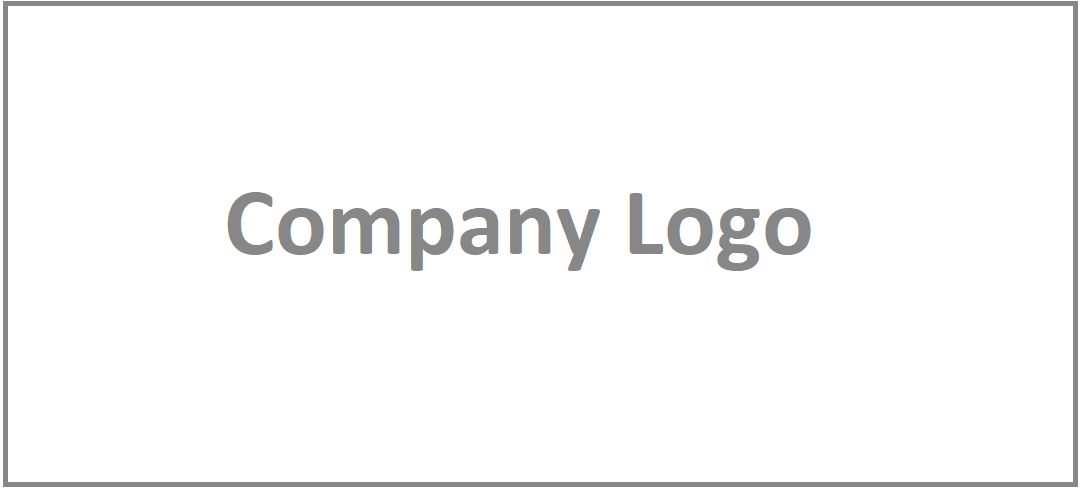
\includegraphics[height=1.5cm]{images/cover/logo-company.png}}
	\chead{}
	\rhead{
\includegraphics[height=1.6cm]{images/cover/logo-dhbw.png}}

	%% Footer
	\lfoot{\documentTypePhrase}
	\cfoot{\documentAuthor}
	\rfoot{Seite | \thepage}

	%% Line between header/footer and text
	\renewcommand{\headrulewidth}{0.4pt}
	\renewcommand{\footrulewidth}{0.4pt}
}


% Include document settings
%!TEX root = ../main.tex

%% Document language (en, de)
\newcommand{\documentLanguage}{de} % Currently not everywhere working

%% Document type
% T3\_1000 Project Thesis (Semester 1 & 2)
% T3\_2000 Project Thesis (Semester 3 & 4, one part)
% T3\_2001 Project Thesis (Semester 3, two parts)
% T3\_2002 Project Thesis (Semester 4, two parts)
% T3\_3000 Project Thesis (Semester 5 & 6)
% T3\_3100 Seminar Paper (Semester 5)
% T3\_3200 Seminar Paper (Semester 6)
% T3\_3300 Bachelor Thesis (Semester 6)
\newcommand{\documentType}{T3\_3300}

\newcommand{\multipleAuthors}{false} % Currently not everywhere working
\newcommand{\documentAuthor}{Author}
\newcommand{\documentTitle}{Title}
\newcommand{\exam}{}
\newcommand{\modul}{}
\newcommand{\documentPeriod}{Juni 20xx bis September 20xx}

\newcommand{\matriculationNumber}{1234567}

\newcommand{\locationUniversity}{Stuttgart}
\newcommand{\department}{Elektrotechnik-Automation}
\newcommand{\course}{TELxxGR4}

\newcommand{\degree}{Bachelor of Engineering}
% INF2014 - INF2016 (MI):       Bachelor of Science
% INF2014 - INF2016 (IA/IM) :   Bachelor of Engineering
% INF2017 (all):                Bachelor of Science

\newcommand{\releaseDate}{xx.xx.20xx}
\newcommand{\releaseLocation}{Company Location}

\newcommand{\companyName}{Company}
\newcommand{\companyLocation}{12345 Location}

\newcommand{\tutor}{Compnay Tutor}
\newcommand{\evaluator}{DHBW Evaluator}


% Load language specific Strings
\input{ads/\documentLanguage}

% Load language specific babel package
\iflang{de}{\usepackage[english, ngerman]{babel}}
\iflang{en}{\usepackage[ngerman, english]{babel}}

% Add comment feature
\newcommand{\comment}[1]{\par {\fontsize{15pt}{15pt} \bfseries \color{red} #1 \par}}


%%%%%%% Package Includes %%%%%%%

\usepackage[margin=\margin,top=20mm,foot=1mm]{geometry}
\usepackage[activate]{microtype}
\usepackage[onehalfspacing]{setspace}
\usepackage{makeidx}
\usepackage[autostyle=true,german=quotes]{csquotes}
\usepackage{longtable}
\usepackage{enumitem}
\usepackage{graphicx}
\usepackage{pdfpages}
\usepackage{color}
\usepackage{xcolor} 	% Chapter/Section color
\usepackage{sectsty}	% Chapter/Section color
\usepackage{float}
\usepackage{array}
\usepackage{calc}
\usepackage[right]{eurosym}
\usepackage{wrapfig}
\usepackage{pgffor}
\usepackage[perpage, hang, multiple, stable]{footmisc}
\usepackage{acronym}%[printonlyused]{acronym}
\usepackage{listings}
\usepackage[obeyFinal,backgroundcolor=yellow,linecolor=black]{todonotes}
\usepackage{rotating}
\usepackage{lscape}
\usepackage{amsmath}
\usepackage{amssymb}
\usepackage[scaled]{uarial}
\usepackage{\documentFont}
\usepackage[%
	pdftitle={\documentTitle},
	pdfauthor={\documentAuthor},
	pdfsubject={\documentType},
	pdfcreator={pdflatex, LaTeX with KOMA-Script},
	pdfpagemode=UseOutlines,       % Show Contents while opening
	pdfdisplaydoctitle=true, 		% Show document title instead of file name
	pdflang={\documentLanguage}, % Document language
]{hyperref}
\usepackage{bookmark}
\usepackage[nonumberlist,toc]{glossaries}
\usepackage{fancyhdr}	% Header and Footer
\usepackage[notindex,nottoc]{tocbibind}	% LoF and LoT in ToC

% Generate glossary
\makeglossaries{}

% Load colors
\defineColors{}
\chapterfont{\color{chapterBlue}}
\sectionfont{\color{chapterBlue}}
\subsectionfont{\color{chapterBlue}}
\subsubsectionfont{\color{chapterBlue}}

% Set Titel, Autor and Date
\title{\documentTitle}
\author{\documentAuthor}
\date{\releaseDate}


% PDF link settings
\hypersetup{%
	colorlinks=false,
	linkcolor=LinkColor,
	citecolor=LinkColor,
	filecolor=LinkColor,
	menucolor=LinkColor,
	urlcolor=LinkColor,
	linktocpage=true,
	bookmarksnumbered=true
}

% Workaround um Fehler in Hyperref, muss hier stehen bleiben
\usepackage{bookmark} %nur ein latex-Durchlauf für die Aktualisierung von Verzeichnissen nötig

% Captions fontsize
\addtokomafont{caption}{\small}

% Bibliographie settings
\iflang{de}{%
	\usepackage[
		backend=biber,		% recommended. Alternative: biblatex
		bibwarn=true,
		bibencoding=utf8,	         % If .bib file is encoded with utf8, otherwise ascii
		sortlocale=de_DE,
		style=\quoteStyle,
	]{biblatex}
}
%\iflang{en}{%
%\usepackage[
%	backend=biber,		% recommended. Alternative: biblatex
%	bibwarn=true,
%	bibencoding=utf8,        % If .bib file is encoded with utf8, otherwise ascii
%	sortlocale=en_US,
%	style=\quoteStyle,
%]{biblatex}
%}
\ladeliteratur
\newcommand{\mkbibnodate}{o\adddot J\adddot}
\AtEveryBibitem{\iffieldundef{year}{\restorefield{year}{\mkbibnodate}}{}}

\usepackage{url}
\def\UrlBreaks{\do\a\do\b\do\c\do\d\do\e\do\f\do\g\do\h\do\i\do\j\do\k\do\l\do\m\do\n\do\o\do\p\do\q\do\r\do\s\do\t\do\u\do\v\do\w\do\x\do\y\do\z\do\0\do\1\do\2\do\3\do\4\do\5\do\6\do\7\do\8\do\9\do\-\do\_} 
\urlstyle{same}

% Hurenkinder und Schusterjungen verhindern
% http://projekte.dante.de/DanteFAQ/Silbentrennung
\clubpenalty = 10000 % schließt Schusterjungen aus (Seitenumbruch nach der ersten Zeile eines neuen Absatzes)
\widowpenalty = 10000 % schließt Hurenkinder aus (die letzte Zeile eines Absatzes steht auf einer neuen Seite)
\displaywidowpenalty=10000

% Graphicspath
\graphicspath{{images/}}

% frequently used programing languages
\lstloadlanguages{PHP,Python,Java,C,C++,bash}

\listingsettings{}
% Rename Listings
\renewcommand\lstlistingname{\listingPhrase}
\renewcommand\lstlistlistingname{\listListingPhrase}
\def\lstlistingautorefname{\authorListingPhrase}

% Spaces in tables
\setlength{\tabcolsep}{\tableColumnMargin}
\renewcommand{\arraystretch}{\tableRowMargin}

%% Header and Footer
\headersettings{}

%% Program name style
\newcommand{\ProgramName}[1]{{\textit{#1}}}

%% Table of contents -> dots
\usepackage{tocloft}
\renewcommand{\cftchapdotsep}{\cftdotsep}
\renewcommand{\cftchapleader}{\cftdotfill{\cftchapdotsep}}

%% Spacing before and after chapter at ToC, LoF, LoT
\setlength{\cftbeforetoctitleskip}{0pt}
\setlength{\cftaftertoctitleskip}{0pt}
\setlength{\cftbeforeloftitleskip}{0pt}
\setlength{\cftafterloftitleskip}{0pt}
\setlength{\cftbeforelottitleskip}{0pt}
\setlength{\cftafterlottitleskip}{0pt}

%% Color of ToC, LoF, LoT
\renewcommand{\cfttoctitlefont}{\color{chapterBlue}\Huge\bfseries}
\renewcommand{\cftloftitlefont}{\color{chapterBlue}\Huge\bfseries}
\renewcommand{\cftlottitlefont}{\color{chapterBlue}\Huge\bfseries}

%\renewcommand{\cftfigpresnum}{Abb. }
%\renewcommand{\cftfignumwidth}{def}


\begin{document}

	% Cover
	\begin{spacing}{1}
		%!TEX root = ../main.tex

\begin{titlepage}
	\begin{longtable}{p{8cm} p{8cm}}
		\raggedright {\raisebox{\ht\strutbox-\totalheight}{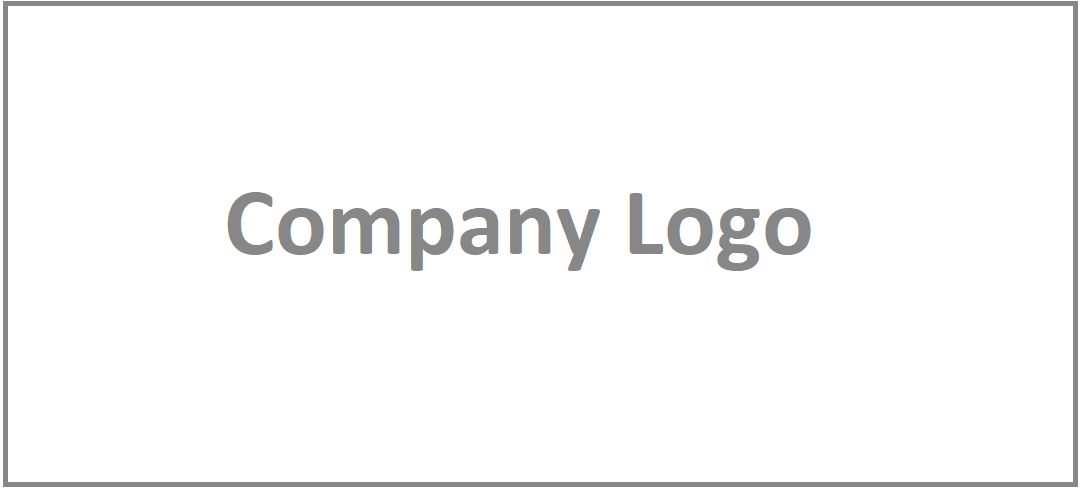
\includegraphics[height=2.0cm]{images/cover/logo-company.png}}} &
		\ifDocType{T2\_3100}{%
			% no company logo for semester paper
		}{%
			\raggedleft {\raisebox{\ht\strutbox-\totalheight}{
\includegraphics[height=2.0cm]{images/cover/logo-dhbw.png}}}
		}%
	\end{longtable}
	%\enlargethispage{20mm}
	\begin{center}
    \doublespacing{
		\vspace*{12mm}	{\LARGE\textbf \documentTitle }}\\
		\vspace*{12mm}	{\large\textbf {\documentTypePhrase}}\\
		\vspace*{12mm}	{\textbf{\exam}}\\
		\vspace*{0mm}	{\textbf{\modul}}\\

		% degre only for bachelor thesis
		\ifDocType{T2\_3300}{
			\vspace*{12mm}	\degreePhrase\\
			\vspace*{3mm}	\textbf{\degree}\\
		}

		\vspace*{12mm}	\departmentPhrase{} \department\\
		\vspace*{0mm}	\locationUniversityPhrase{} \locationUniversity\\
		\vspace*{12mm}	\documentAuthorPhrase\\
		\vspace*{3mm}	{\large\textbf \documentAuthor}\\
		\vspace*{12mm}	\releaseDate\\
	\end{center}
	\vfill
	\begin{spacing}{1.2}
	\begin{tabbing}
		mmmmmmmmmmmmmmmmmmmmmmmmmm             \= \kill
		\textbf{\documentPeriodPhrase} \> \documentPeriod\\
		\textbf{\matriculationNumberPhrase, \coursePhrase}  \>  \matriculationNumber, \course\\

		\ifDocType{T3\_3100}{%
			% no company for the semester paper 1
		}{%
			\ifDocType{T3\_3200}{%
				% no company for the semester paper 2
			}{%
				\textbf{\companyPhrase}                  \>  \companyName, \companyLocation\\
			}%
		}%
		\textbf{\tutorPhrase}               \>  \tutor\\

		% evaluator only for bachelor thesis
		\ifDocType{T3\_3300}{%
			\textbf{\evaluatorPhrase}              \>  \evaluator
		}{}
	\end{tabbing}
	\end{spacing}
\end{titlepage}

	\end{spacing}
	\newpage

	\pagestyle{fancy}
	\fancypagestyle{plain}{}
	\pagenumbering{Roman}

	% Restriction notices
	\ifDocType{T3\_3100}{%
		% no restricition notices for semester paper 1
	}{%
		\ifDocType{T3\_3200}{%
			% no restricition notices for semester paper 2
		}{%
			%!TEX root = ../main.tex

%\thispagestyle{empty}

\section*{\restrictionNoticesPhrase}

\iflang{de}{
	Die vorliegende {\documentTypePhrase} mit dem Titel "`{\textit{\documentTitle}}"' beinhaltet unternehmensinterne, vertrauliche Informationen der {\companyName}. Die Arbeit wird ausschließlich für Prüfungszwecke an der Dualen Hochschule Baden-Württemberg {\locationUniversity} vorgelegt. Die Weitergabe des Inhaltes der Arbeit, beiliegender Zeichnungen und Daten im Gesamten oder in Teilen ist Grundsätzlich untersagt.
	Es dürfen keinerlei Kopien oder Abschriften - auch in digitaler Form - angefertigt werden. Ausnahmen bedürfen der schriftlichen Genehmigung der {\companyName} und des Verfassers.% \\

%  Die vorliegende {\documentTypePhrase} mit dem Titel {\itshape{}\documentTitle{}\/} enthält
%  unternehmensinterne bzw. vertrauliche Informationen der {\companyName}, ist deshalb mit einem
%  Sperrvermerk versehen und wird ausschließlich zu Prüfungszwecken am Studiengang {\department}
%  der Dualen Hochschule Baden-Württemberg {\locationUniversity} vorgelegt. Sie ist ausschließlich zur
%  Einsicht durch den zugeteilten Gutachter, die Leitung des Studiengangs und ggf. den Prüfungsausschuss
%  des Studiengangs bestimmt.  Es ist untersagt,
%  \begin{itemize}
%  \item den Inhalt dieser Arbeit (einschließlich Daten, Abbildungen, Tabellen, Zeichnungen usw.) als
%            Ganzes oder auszugsweise weiterzugeben,
%  \item Kopien oder Abschriften dieser Arbeit (einschließlich Daten, Abbildungen, Tabellen,
%             Zeichnungen usw.) als Ganzes oder in Auszügen anzufertigen,
%  \item diese Arbeit zu veröffentlichen bzw. digital, elektronisch oder virtuell zur Verfügung zu stellen.
%  \end{itemize}
%Jede anderweitige Einsichtnahme und Veröffentlichung – auch von Teilen der Arbeit – bedarf der
%vorherigen Zustimmung durch den Verfasser und {\companyName}.
}

%\releaseLocation, \releaseDate
%\vspace{2em}
%
%\rule{6cm}{0.4pt}\\
%\documentAuthor

%			\newpage
		}%
	}%

	% Declaration
	%!TEX root = ../main.tex

%\thispagestyle{empty}

\section*{\declarationPhrase}

\iflang{de}{
	Gemäß § 5 (3) der "`Studien- und Prüfungsordnung für Bachelorstudiengänge im Studienbereich Technik der Dualen Hochschule Baden-Württemberg"' vom 29. September 2017.\\
	\\
	Hiermit versichere ich, dass die vorliegende Arbeit mit dem Titel "`{\textit{\documentTitle}}"' selbstständig verfasst und keine anderen als die angegebenen Quellen und Hilfsmitteln verwendet habe.
	% Ich versichere zudem, dass die eingereichte elektronische Fassung mit der gedruckten Fassung übereinstimmt. \\
%  \ifMultipleAuthors{Wir versichern}{Ich versichere} hiermit, dass \ifMultipleAuthors{wir unsere}{ich meine}
%  {\documentTypePhrase} mit dem Thema: {\itshape \documentTitle }
%  selbstständig verfasst und  keine anderen als die angegebenen Quellen und Hilfsmittel benutzt \ifMultipleAuthors{haben}{habe}.
%  \ifMultipleAuthors{Wir versichern}{Ich versichere} zudem, dass die eingereichte elektronische Fassung mit der gedruckten Fassung
%  übereinstimmt.
}

\releaseLocation, \releaseDate
\vspace{2em}

\rule{6cm}{0.4pt}\\
\documentAuthor

%	\newpage

	% Anmerkung zum Genus des Substantivs
	%!TEX root = ../main.tex

\section*{Anmerkung zum Genus des Substantivs}

Auf geschlechtsspezifische Umschreibung ist hier verzichtet worden. Ein Maskulinum - wie zum Beispiel der Student - meint (selbstredend) auch weibliche und diverse Personen.

	\newpage

	% Abstract
	%!TEX root = ../main.tex

%\pagestyle{empty}

\section*{Zusammenfassung / Abstract}

deutsch \\
\\
\textit{englisch}

	\newpage

	% Table of contents
	\begin{spacing}{1.5}
		\begingroup
		    % set subchapter depth
			\setcounter{tocdepth}{2}
			\tableofcontents
			\clearpage
		\endgroup
	\end{spacing}
	\newpage

	% Acronyms
	\cleardoublepage
	%!TEX root = ../main.tex

\addchap{\acronymsPhrase}

\begin{acronym}%s[RedBox] % Längstes Acronymm
%\setlength{\itemsep}{-\parsep} %kein Abstand, kompakte Darstellung
% Von Hand sortieren, automatisch mit CMD: sort file.txt /O file.txt

\acro{DHBW}{Dualen Hochschule Baden-Württemberg}

\end{acronym}


	\pagenumbering{arabic}

	% Content
	\acresetall
	%!TeX encoding = UTF-8
%!TEX root = ../main.tex

\input{chapter/Einführung.tex}


	\clearpage

	% Glossar
%	\cleardoublepage
%	\printglossary[style=altlist,title=\glossaryPhrase]
%	%!TEX root = ../main.tex

%
% To create glossary run the following command:
% makeglossaries main.acn && makeglossaries main.glo
%

%
% Glossareintraege --> referenz, name, beschreibung
% Aufruf mit \gls{...}
%
\newglossaryentry{Glossareintrag}{name={Glossareintrag},plural={Glossareinträge},description={Ein Glossar beschreibt verschiedenste Dinge in kurzen Worten}}


	% Bibilography
%	\clearpage
	\printbibliography[title=Literaturverzeichnis]

	% List of Figures
	\cleardoublepage
	\listoffigures

	% List of Tables
	\cleardoublepage
	\listoftables

	% List of Listings
	\begingroup
	\let\clearpage\relax
%		\cleardoublepage
		\lstlistoflistings
	\endgroup

	% Appendix
%	\clearpage
	\appendix
	%!TeX root = ../main.tex

% Disable \clearpage
\begingroup
\let\clearpage\relax

\addchap{\appendixPhrase}

\begin{itemize}
	\item \ref{apx:doku} Anhang 1
\end{itemize}

% Enable \clearpage
\endgroup

\chapter{Anhang 1}
\label{apx:doku}
%\includepdf[pages=-]{chapter/appendix.pdf}


\end{document}
